\section{Progress}
\label{sec:progress}

\begin{frame}
  \frametitle{Coordinate Transformation - ex: 359711}
  These configurations all match a beam configuration that should yield similar
  results. The simulations are set up for half-scans - therefore, we need to
  apply the proper transformation to get the correct results from the
  simulation for y-displacements.
  \begin{center}
    \begin{tabular}{c c c c c c}
      \toprule
      \textbf{$\Delta$}
      & \textbf{$\theta_{xing}$}
      & \textbf{$(\Delta)_t$}
      & \textbf{$(\theta_{xing})_t$} \\
      \midrule
        -1000$\mu$m, x & 0.06E-3 & N/A           & N/A \\
         1000$\mu$m, x & 0.1 E-3 & 1000$\mu$m, x & '-' \\
        -1000$\mu$m, y & 0.06E-3 &-1000$\mu$m, x & '-' \\
         1000$\mu$m, y & 0.07E-3 &-1000$\mu$m, x & '-' \\
      \bottomrule
    \end{tabular}
  \end{center}
\end{frame}

\begin{frame}
  \frametitle{Coordinate Transformation - ex: 359711}
  This tells us that we can freely substitute y for x, and should not expect to
  cover any issues up. We showed in earlier work that the $\theta_{xing}$
  probably only occurs in the X-Z plane, and that X-Z crossing angles
  independently affect the z-vertex profile from Y-Z crossing angles.
  Plots follow.
  \begin{center}
    \begin{tabular}{c c c c c c}
      \toprule
      \textbf{$\Delta$}
      & \textbf{$\theta_{xing}$}
      & \textbf{$(\Delta)_t$}
      & \textbf{$(\theta_{xing})_t$} \\
      \midrule
      -1000$\mu$m, x & 0.06E-3 & N/A           & N/A \\
      1000$\mu$m, x & 0.1 E-3 & 1000$\mu$m, x & '-' \\
      -1000$\mu$m, y & 0.06E-3 &-1000$\mu$m, x & '-' \\
      1000$\mu$m, y & 0.07E-3 &-1000$\mu$m, x & '-' \\
      \bottomrule
    \end{tabular}
  \end{center}
\end{frame}

\begin{frame}
  \frametitle{359711 - Step 00, -1000$\mu$m}
  \begin{center}
    \begin{figure}
      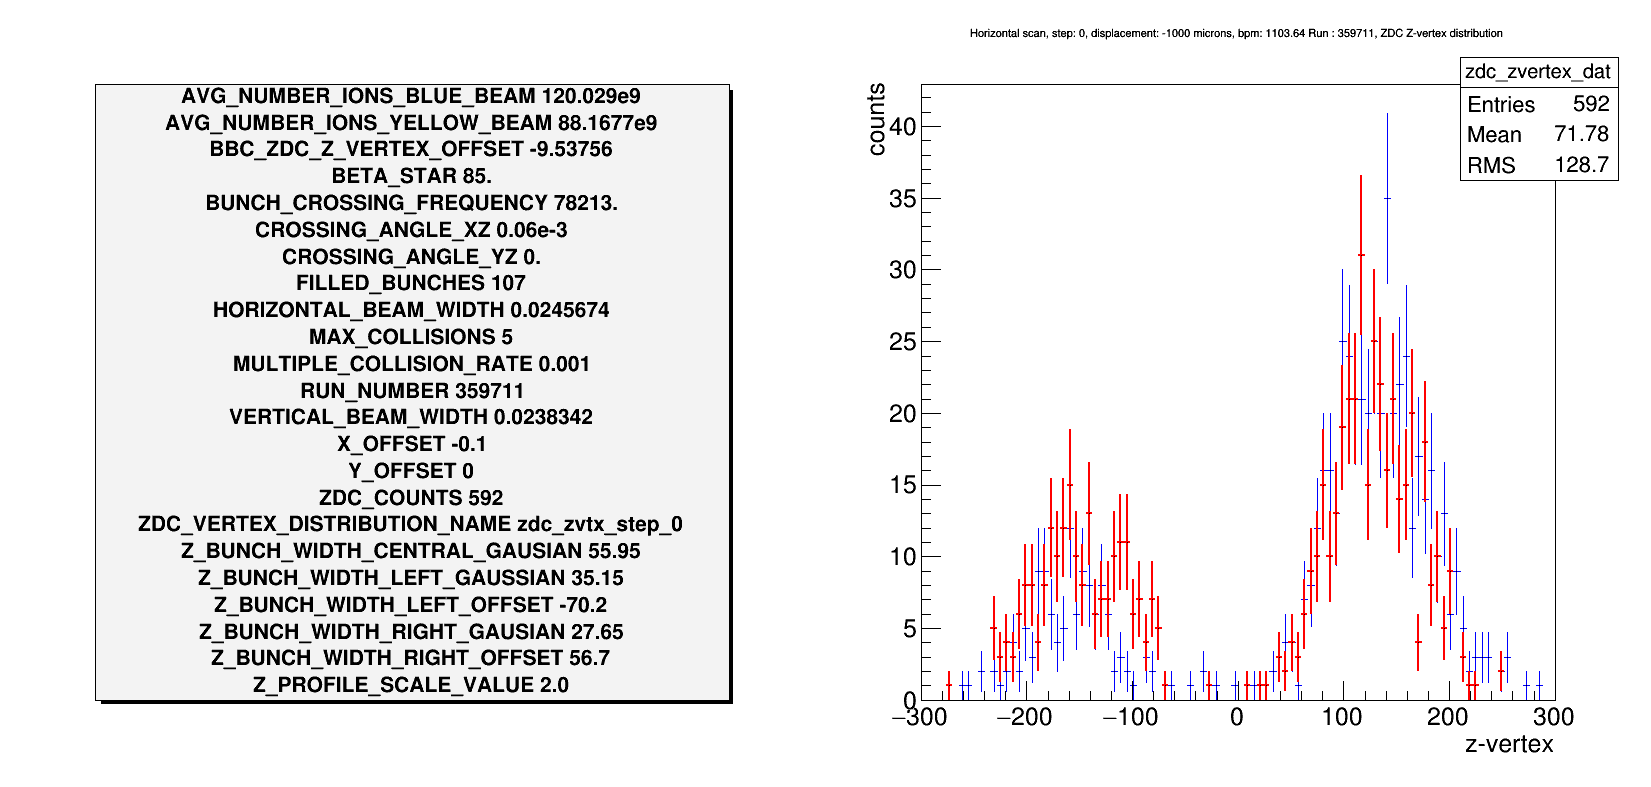
\includegraphics[width=\linewidth]{./figures/step_00_transf}
      \caption{
        By-eye matching to understand if we can simply swap x, y for y-scan
        steps to ensure no special care is needed with transformations. This is
        the horizontal scan, step 00, -1000 microns.
      }
      \label{fig:step_00_transf}
    \end{figure}
  \end{center}
\end{frame}

\begin{frame}
  \frametitle{359711 - Step 12, 1000$\mu$m}
  \begin{center}
    \begin{figure}
      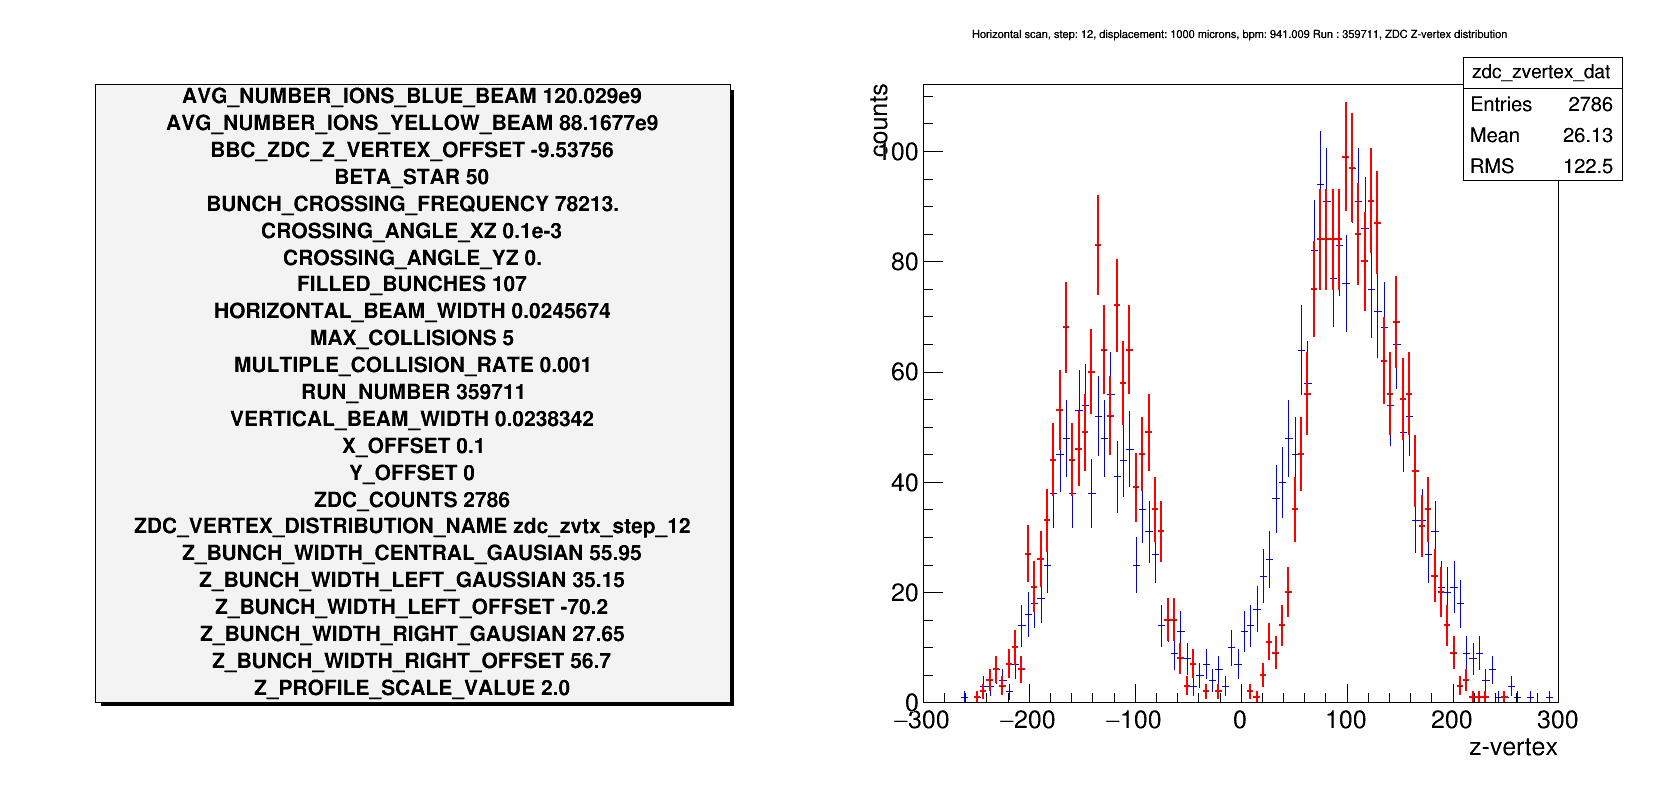
\includegraphics[width=\linewidth]{./figures/step_12_transf}
      \caption{
        By-eye matching to understand if we can simply swap x, y for y-scan
        steps to ensure no special care is needed with transformations. This is
        the horizontal scan, step 12, 1000 microns.
      }
      \label{fig:step_12_transf}
    \end{figure}
  \end{center}
\end{frame}

\begin{frame}
  \frametitle{359711 - Step 13, -1000$\mu$m}
  \begin{center}
    \begin{figure}
      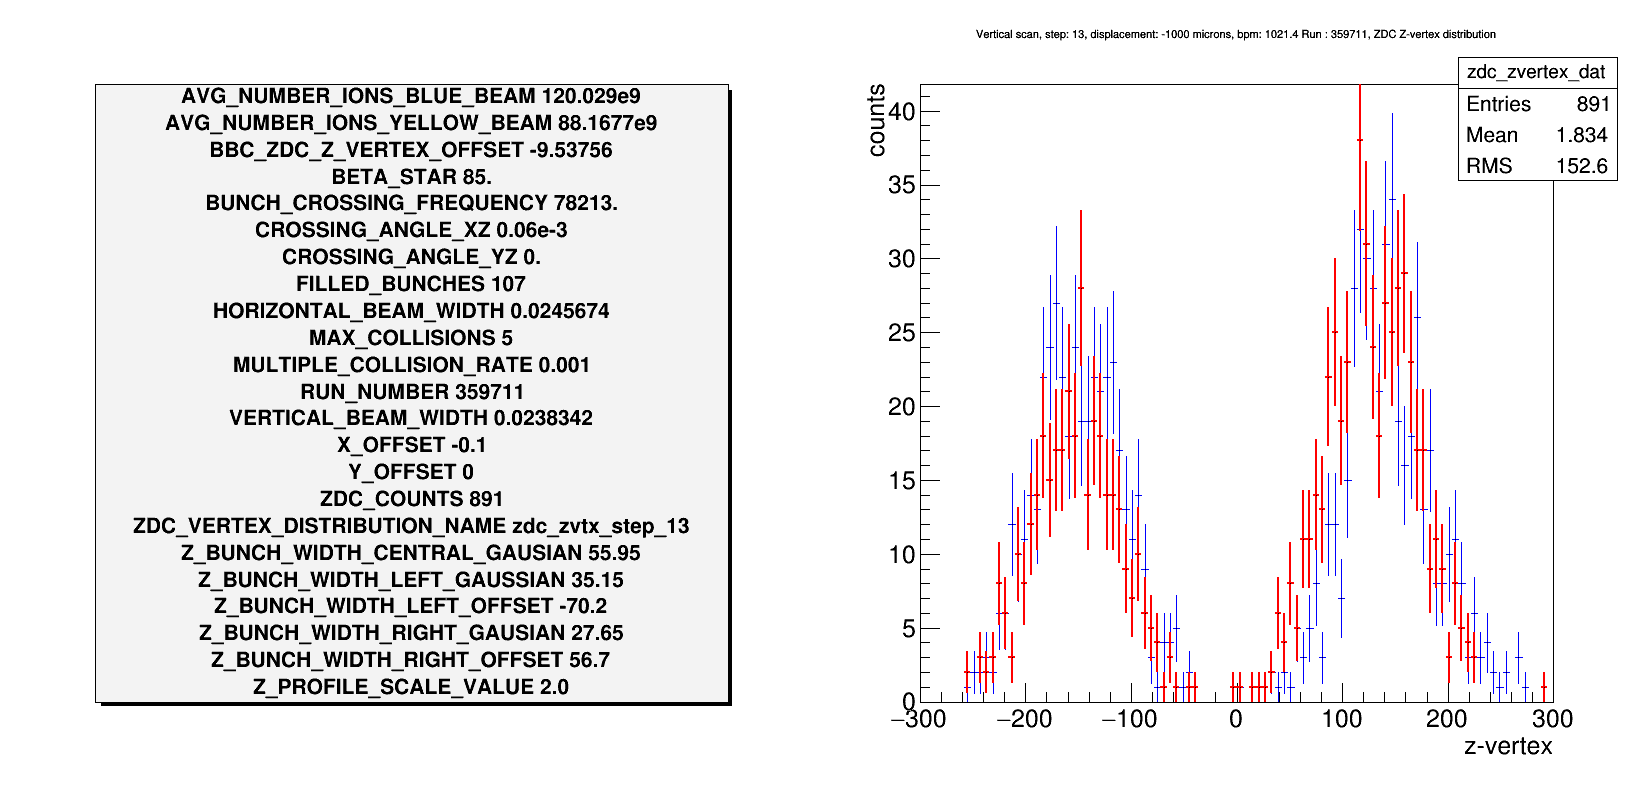
\includegraphics[width=\linewidth]{./figures/step_13_transf}
      \caption{
        By-eye matching to understand if we can simply swap x, y for y-scan
        steps to ensure no special care is needed with transformations. This is
        the vertical scan, step 13, -1000 microns. We can see that the
        distributions match well and will proceed.
      }
      \label{fig:step_12_transf}
    \end{figure}
  \end{center}
\end{frame}

\begin{frame}
  \frametitle{359711 - Step 25, 1000$\mu$m}
  \begin{center}
    \begin{figure}
      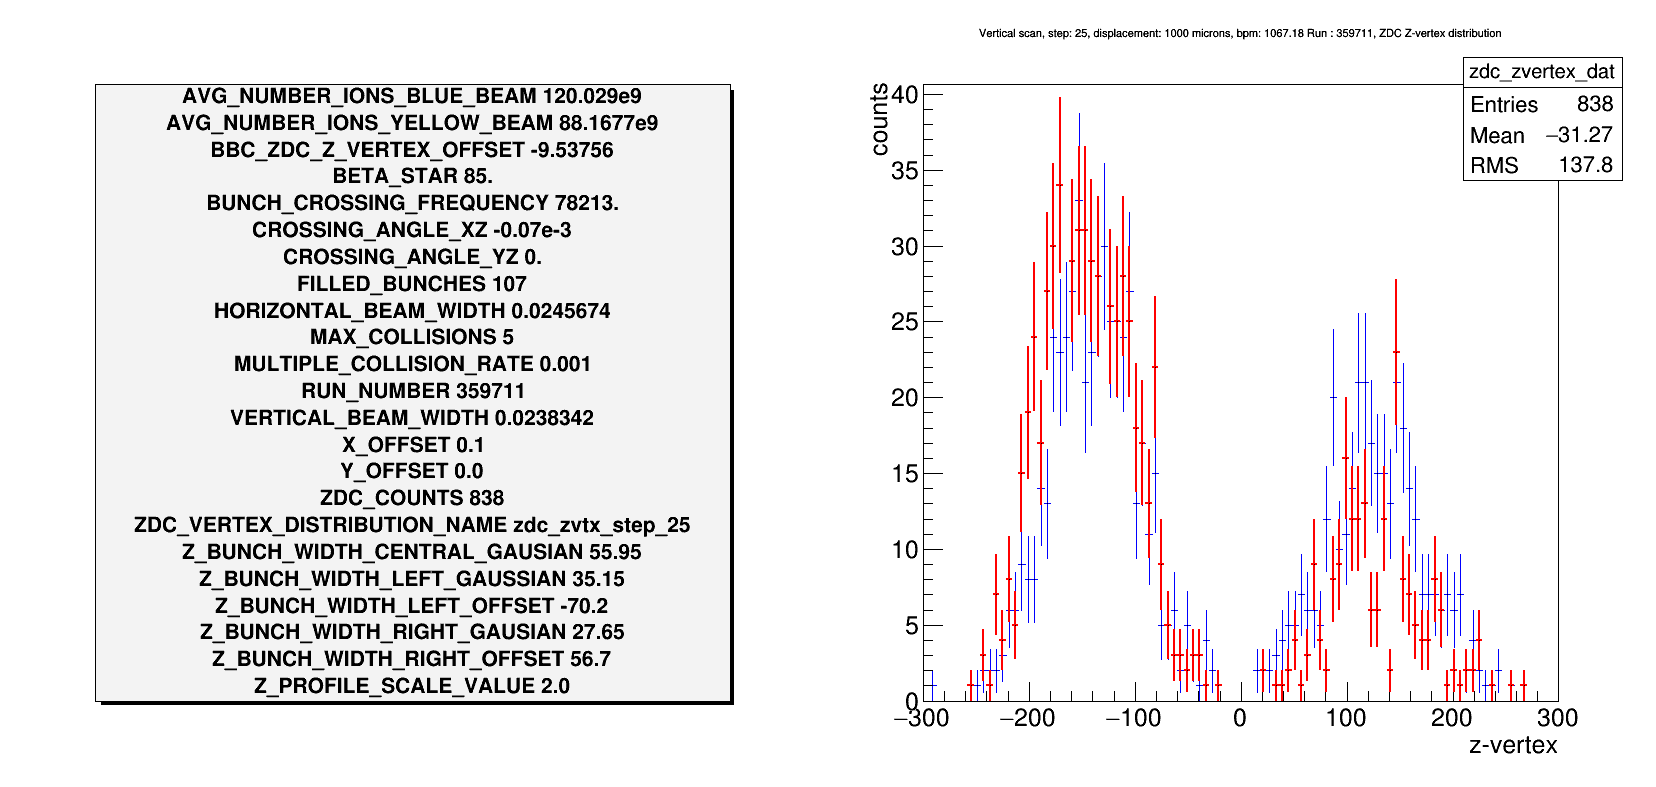
\includegraphics[width=\linewidth]{./figures/step_25_transf}
      \caption{
        By-eye matching to understand if we can simply swap x, y for y-scan
        steps to ensure no special care is needed with transformations. This is
        the vertical scan, step 25, 1000 microns. We can see that distributions
        match well, and will proceed.
      }
      \label{fig:step_12_transf}
    \end{figure}
  \end{center}
\end{frame}
